\documentclass[../main.tex]{subfiles}
\begin{document}
\chapter{Inhomogeneous Problems and Green's Functions}
\section{Dirac Delta Function}
\subsection{Defining a Delta Function} \cref{deltaDef}
In IA Differential equations we saw a ``function'' $\delta(x)$ with:
\[
  \delta(x) = 0\ \forall x \neq 0 \text{ and } \int_{-\varepsilon}^{\varepsilon} \delta(x) \d{x} = 1\ \forall \varepsilon > 0
\]
and a \textit{sampling property}:
\[
  \int_{-\infty}^{\infty} \delta(x - a)f(x) \d{x} = f(a)
\]
But how can we make sense of such a $\delta(x)$?

We define the sequence of functions $\{\delta_n\}^{n = 1}_{\infty}$ by:
\[
  \delta_n(x) = \begin{cases}
  \frac{n}{\alpha}\exp\left[-\frac{1}{1 - (nx)^2}\right] & |x| < \frac{1}{n} \\
  0 & |x| \geq \frac{1}{n}
  \end{cases}
\]
where:
\[
  \alpha = \int_{-1}^{1} \exp\left[-\frac{1}{1 - y^2}\right] \d{y}
\]
Graphically, these look like:
\begin{center}
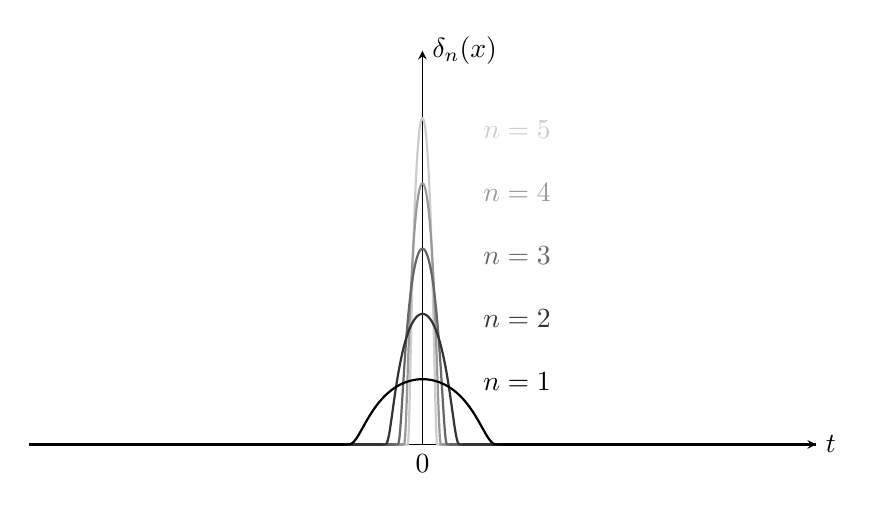
\begin{tikzpicture}[>=stealth]
  \draw[->] (-5, 0) -- (5, 0) node[right] {$t$};
  \draw[->] (0, 0) node[below] {0} -- (0, 5) node[right] {$\delta_n(x)$};
  \def\aconst{0.443993816168}

  \foreach \op/\nconst in {20/5, 40/4, 60/3, 80/2, 100/1} {
    \draw[thick, domain=-(1/\nconst) + 0.001:(1/\nconst) - 0.001, smooth, samples=100, black!\op] plot (\x,{(\nconst/\aconst) * exp(1/((\nconst * \x)^2 - 1))});
    \node[black!\op] at (1.2, 0.8 * \nconst) {$n = \nconst$};
    \draw[thick, black!\op] (-5, 0) -- (-1/\nconst, 0);
    \draw[thick, black!\op] (1/\nconst, 0) -- (5, 0);
  }
\end{tikzpicture}
\end{center}
This sequence has the following properties:
\begin{enumerate}
  \item $\delta_n(x)$ is smooth for all $n \in \N$
  \item $\delta_n(x) = 0$ outside of $(-1/n, 1/n)$
  \item For all $\varepsilon > 0$, there exists $N$ such that for all $n \geq N$:
    \[
      \int_{-\varepsilon}^{\varepsilon} \delta_n(x) \d{x} = 1
    \]
    This follows from taking $N \geq 1/\varepsilon$ so that for $n \geq N$, the support of $\delta_n$ is within $(-\varepsilon, \varepsilon)$ so that:
    \begin{align*}
      \int_{-\varepsilon}^{\varepsilon} f_n(x) \d{x} &= \int_{-1/n}^{1/n} f_n(x) \d{x} \\
                                                     &= \int_{-1/n}^{1/n} \frac{n}{\alpha} \exp\left[-\frac{1}{1 - (n x)^2}\right] \d{x} \\
                                                     &= \int_{-1}^{1} \frac{1}{\alpha} \exp\left[-\frac{1}{1 - y^2}\right] \d{x} \\
                                                     &= 1
    \end{align*}
\end{enumerate}
With this sequence of functions, we have pointwise limits at $x \neq 0$:
\[
  \lim_{n \to \infty} \delta_n(x) = 0 \text{ for $x \neq 0$}
\]
and:
\[
  \lim_{n \to \infty} \int_{-\varepsilon}^{\varepsilon} \delta_n(x) \d{x} = 1\ \forall \varepsilon > 0
\]
So it \textit{almost} looks like $\delta(x) = \lim_{n \to \infty} \delta(x)$.
The limit does not exist in the pointwise sense as $\lim_{n \to \infty} \delta_n(0)$ diverges, however it does exist in a weaker sense.

We note that delta functions rarely exist in isolation and usually appear inside integrals or as a forcing term in a differential equation.
For example:
\[
  \int_{-\infty}^{\infty} \delta(x - a)f(x) \d{x} \text{ and } \ddot{y} + \omega^2 y = \delta(t)
\]
To utilise $\delta_n$, we will think of these as \textit{sequences of statements} indexed in $n$, each yielding a result which we will take the limit of.
In the above example, we interpret the sampling integral as the following:
\[
  \int_{-\infty}^{\infty} \delta(x - a) f(x) \d{x} = \lim_{n \to \infty} \int_{-\infty}^{\infty} \delta_n(x - a) f(x) \d{x}
\]
Here, since the integral is done \textit{before} the limit, we do not need to worry about the limit of $\delta_n$ at $0$.
Similarly for the differential equation:
\[
  \ddot{y}_n + \omega^2 y_n = \delta_n(t)
\]
which has a solution $y_n$ for each $n$.
We then interpret the solution to the original differential equation as:
\[
  y(t) = \lim_{n \to \infty} y_n(t)
\]
This framework even allows us to deal with $\delta'(x)$:
\begin{align*}
  \int_{-\infty}^{\infty} \delta'(x)f(x) \d{x} &= \lim_{n \to \infty} \int_{-\infty}^{\infty} \delta'_n(x) f(x) \d{x} \\
                                               &= \lim_{n \to \infty} \left(\eval{\delta_n(x) f(x)}{-\infty}{\infty} - \int_{-\infty}^{\infty} \delta_n(x) f'(x) \d{x}\right) \\
                                               &= - \lim_{n \to \infty} \int_{-\infty}^{\infty} \delta_n(x) f'(x) \d{x} \\
                                               &= - \int_{-\infty}^{\infty} \delta(x)f'(x) \d{x} \\
                                               &= -f'(0)
\end{align*}
Dealing with these limits every time we would like to utilise a $\delta$ becomes tedious and so we tend to just ignore them.
We can then manipulate $\delta$ like an ordinary function, knowing that we are just manipulating the sequence of statements involving $\delta_n$ for each $n$.
\subsection{Fourier Series}
We define the \textit{L-periodic $\delta$ function}, $\delta^{L}$, as:
\[
  \delta^{L}(x) = \delta(x) \text{ on } x \in \left[-\frac{L}{2}, \frac{L}{2}\right)
\]
which we extend to an $L$-periodic function on $\R$.
Since this is a periodic function, we can compute its Fourier coefficients:
\[
  \left(\hat{\delta}\right)_n = \frac{1}{L} \int_{-L/2}^{L/2} \delta(x)e^{-2\pi i n x/L} \d{x} = \frac{1}{L}
\]
Thus $\delta^{L}$ has Fourier series:
\[
  \delta^{L}(x) \sim \sum_{n \in \Z} \frac{1}{L} e^{2\pi i n x/L}
\]
We expect that since $\delta = \delta^{L}$ on $[-L/2, L/2)$ that $\delta^{L}$ would also have the sampling property of $\delta$, that is:
\[
  f(0) = \int_{-L/2}^{L/2} \delta^{L}(x)f(x) \d{x}
\]
To check this:
\begin{align*}
  \int_{-L/2}^{L/2} \delta^{L}(x)f(x) \d{x} &= \int_{-L/2}^{L/2} \frac{1}{L} \sum_{n \in \Z} e^{2 \pi i n x/L} \d{x} \\
                                            &= \sum_{n \in \Z} \left[\frac{1}{L} \int_{-L/2}^{L/2} f(x) e^{2\pi i n x/L} \d{x}\right] \\
                                            &= \sum_{n \in \Z} \hat{f}_{-n} \\
                                            &= \sum_{n \in \N} \hat{f}_n
\end{align*}
If $f$ is sufficiently nice (i.e. it satisfies the conditions for \cref{convFourier}), then $f(x) = \sum_{n \in \Z} \hat{f}_n e^{2 \pi i n x/L}$ for $x \in [-L/2, L/2)$, that is:
\[
  \int_{-L/2}^{L/2} \delta^{L}(x)f(x) \d{x} = \sum_{n \in \N} \hat{f}_n = f(0)
\]
\subsection{Eigenfunction Expansions}
Consider the Sturm-Liouville problem $\mathcal{L} y = \lambda y$ on the usual vector space from \cref{selfAdjAndBCs}:
\[
  V = \{y \in C^2([a, b]): \text{$y$ satisfies real homogeneous B.C.s at non-singular endpoints}\}
\]
Let $\{Y_k\}^{\infty}_{k = 1}$ be the \textbf{normalised} eigenfunctions of $\mathcal{L}$.
Fix $\xi \in (a, b)$ and consider $g_n(x) = \delta_n(x - \xi)$.
By construction, for $n$ sufficiently large, the support of this function is entirely within $(a, b)$ and has value and derivatives all zero at the endpoints at $a$ and $b$.
Thus $g_n$ will always satisfy homogeneous boundary conditions and the endpoints of $(a, b)$, i.e. $g_n \in V$ for each $n$.

So by \cref{selfAdjProp}, for each $n$, $g_n$ will have an eigenfunction expansion:
\[
  g_n(x) = \delta_n(x - \xi) = \sum_{k = 1}^{\infty} \langle g_n, Y_k \rangle_w Y_k(x)
\]
Where:
\begin{align*}
  \langle g_n, Y_k \rangle_w &= \int_{a}^{b} \delta_n(t - \xi)Y_k(t) w(t)\d{t} \\
                           &\to Y_k(\xi) w(\xi) \text{ as $n \to \infty$}
\end{align*}
Thus, taking $n \to \infty$ on both sides:
\[
  \delta(x - \xi) = \sum_{k = 1}^{\infty} w(\xi)Y_k(\xi)Y_k(x)
\]
For $f \in V$, we would hope that this expansion has the sampling property, i.e.:
\[
  \int_{a}^{b} \delta(x - \xi) f(\xi) \d{\xi} = f(x)
\]
To check this:
\begin{align*}
  \int_{a}^{b} \delta(x - \xi) f(\xi) \d{\xi} &= \int_{a}^{b} [f(\xi) \sum_{n = 1}^{\infty} w(\xi) Y_k(\xi) Y_k(x)] \d{\xi} \\
                                              &= \sum_{n = 1}^{\infty} \left[\int_{a}^{b} f(\xi)Y_k(\xi)w(\xi) \d{\xi}\right] Y_k(x) \\
                                              &= \sum_{k = 1}^{\infty} \langle f,Y_k \rangle_w Y_k(x) \\
                                              &= \sum_{k = 1}^{\infty} \hat{f}_k Y_k(x) \\
                                              &= f(x)
\end{align*}
where $\hat{f}_k$ is the generalised Fourier coefficient (from \cref{generalisedFourier}) $\hat{f}_k = \langle f, Y_k \rangle_{w}$ since $\norm{Y_k}_w = 1$.
\section{Green's Functions}
\subsection{Finding Green's Functions}
\subsubsection{Motivation}
Suppose that we want to solve the BVP:
\begin{equation}
  \label{genSL}
  \begin{cases}
  \mathcal{L}y = f & \text{ for } x \in (a, b) \\
  y(a) = y(b) = 0 &  \\
  \end{cases}
\end{equation}
As we have seen, we can equivalently formulate this as solving $\mathcal{L} y = f$ for $y \in V$ where:
\[
  V = \{y \in C^2([a, b]): y(a) = y(b) = 0\}
\]
Suppose now that $\mathcal{L}$ is a second-order ordinary differential operator, i.e. it can be written as:
\[
  \mathcal{L} = \alpha(x) \deriv[2]{}{x} + \beta(x) \deriv{}{x} + \gamma(x)
\]
where $\alpha, \beta, \gamma$ are smooth and $\alpha(x) \neq 0$ on $(a, b)$.

Fix some $\xi \in (a, b)$.
Suppose that we can find a function $G(x, \xi)$ such that:
\[
  \begin{cases}
  \mathcal{L} G = \delta(x - \xi) & \text{ for } x \in (a, b) \\
  G(a, \xi) = G(b, \xi) = 0 &
  \end{cases}
\]
Given such a $G$, suppose we define $y(x)$ as:
\[
  y(x) = \int_{a}^{b} G(x, \xi) f(\xi) \d{\xi}
\]
then $y(a) = y(b) = 0$ and upon applying $\mathcal{L}$:
\begin{align*}
  \mathcal{L} y &= \int_{a}^{b} f(\xi) \mathcal{L}[G(x, \xi)] \d{\xi} \\
                &= \int_{a}^{b} f(\xi) \delta(x - \xi) \d{\xi} \\
                &= f(x)
\end{align*}
Thus $y$ is a solution to \cref{genSL}.
We call $G(x, \xi)$ the \textit{Dirichlet Green's Function} for $\mathcal{L}$.
But how can we find such $G$?

\subsubsection{Properties of $G(x, \xi)$}
To guide our search, it is first useful to consider what properties $G$ would have if it were to exist.
When $x \in (a, b) \setminus \{\xi\}$, then:
\[
  \mathcal{L}[G(x, \xi)] = \alpha(x) \deriv[2]{G}{x} + \beta(x) \deriv{G}{x} + \gamma(x)G = 0
\]
This is a second order ODE with ``nice'' coefficients and so we expect $x \mapsto G(x, \xi)$ to be ``nice'' away from $x = \xi$.

But what about near $x = \xi$, how can we pick $G$ so that we get $\delta(x - \xi)$ on the right hand side?
Clearly the second order derivative is least regular term on the left hand side and so we want:
\[
  \alpha(x) \deriv{}{x}\left[\deriv{G}{x}(x, \xi)\right] = \delta(x - \varepsilon) + \text{``more regular terms''}
\]
Recall from \cref{deltaDef}, that we can handle $\delta$ more rigorously by considering a sequence of functions $\{\delta_n(x)\}^{n = 1}_{\infty}$.
Using this, we want to look for a sequence of $H_n(x)$ such that:
\[
  \deriv{}{x}[H_n(x)] = \delta_n(x) \text{ for each } n \in \N
\]
Since $\delta_n$ are just normal smooth functions, we can pick $H_n(x)$ as:
\[
  H_n(x) = \int_{-\infty}^{x} \delta_n(t) \d{t}
\]

By how $\delta_n$ were constructed, for any $x > 0$, there exists $N$ such that the support of $\delta_n$ lies entirely within $(-x, x)$ for all $n \geq N$.
Thus:
\[
  H_n(x) = \int_{-\infty}^{x} \delta_n(t) \d{t} = \int_{-1/n}^{1/n} \delta_n(t) \d{t} = 1\ \forall n \geq N
\]
For any $x < 0$, then there exists $N$ such that the support of $\delta_n$ lies entirely within $(x, -x)$ for all $n \geq N$.
Thus:
\[
  H_n(x) = \int_{-\infty}^{x} \delta_n(t) \d{t} = 0\ \forall n \geq N
\]

So interpreting the $\delta$ function as we did in \cref{deltaDef}, for any $x \neq 0$:
\[
  H(x) = \lim_{n \to \infty} H_n(x) = \begin{cases}
  1 & \text{ if } x > 0 \\
  0 & \text{ if } x< 0
  \end{cases}
\]
with $H'(x) = \delta(x)$ where $H$ the called the \textit{Heaviside step function}.
Thus:
\[
  \deriv{}{x}[H(x - \xi)] = \delta(x - \xi)
\]

So we want $\deriv{G}{x}(x, \xi)$ to resemble $H(x - \xi)$ near $x = \xi$, i.e. we expect $\deriv{G}{x}(x, \xi)$ to have a jump discontinuity at $x = \xi$.
Since $G(a, \xi) = 0$, we can write:
\[
  G(x, \xi) = \int_{a}^{x} \deriv{G}{t}(t, \xi) \d{t}
\]
If we try a similar integral on $H(x - \xi)$, then:
\[
  \int_{a}^{x} H(t - \xi) \d{t} = \begin{cases}
  x - \xi & \text{ if } x > \xi \\
  0 & \text{ if } x < \xi
  \end{cases}
\]
which is a continuous function at $x = \xi$ and so we expect $x \mapsto G(x, \xi)$ to be continuous at $x = \xi$.

How can we find the nature of the jump discontinuity in $\deriv{G}{x}$ at $x = \xi$?
If we divide $\mathcal{L} G = \delta(x - \xi)$ by $\alpha \neq 0$ and then integrate $x$ over $(\xi - \varepsilon, \xi + \varepsilon)$ we obtain:
\begin{align*}
  \eval{\deriv{G}{x}}{x = \xi - \varepsilon}{x = \xi + \varepsilon} + \int_{\xi - \varepsilon}^{\xi + \varepsilon} \left[\frac{\beta}{\alpha} \deriv{G}{x} + \frac{\gamma}{\alpha} G\right]\d{x} = \int_{\xi - \varepsilon}^{\xi + \varepsilon} \frac{\delta(x - \xi)}{\alpha(x)} \d{x} = \frac{1}{\alpha(\xi)}
\end{align*}
We know that, at worst, $\deriv{G}{x}$ has a jump discontinuity at $\xi$ and so as $\varepsilon \to 0^{+}$:
\[
   \int_{\xi - \varepsilon}^{\xi + \varepsilon} \left[\frac{\beta}{\alpha} \deriv{G}{x} + \frac{\gamma}{\alpha} G\right]\d{x} \to 0
\]
Thus, the jump discontinuity at $x = \xi$ must satisfy:
\[
  \eval{\deriv{G}{x}(x, \xi)}{x = \xi^{-}}{x = \xi^{+}} = \frac{1}{\alpha(\xi)}
\]

\subsubsection{Summary}
In summary, if $\mathcal{L}G = \delta(x - \xi)$, then $G$ will have the following properties:
\begin{itemize}
  \item $G(x, \xi)$ is continuous at $x = \xi$
  \item $\deriv{G}{x}(x, \xi)$ has a jump discontinuity at $x = \xi$ satisfying:
    \[
      \deriv{G}{x}(\xi^{+}, \xi) - \deriv{G}{x}(\xi^{-}, \xi) = \frac{1}{\alpha(\xi)}
    \]
\end{itemize}
\begin{example}
  Consider the differential operator:
  \[
    \mathcal{L} = \deriv[2]{}{x} + \omega^2
  \]
  for fixed $\omega \in \R$ on the domain $(0, 1)$.
  We would like to find the Dirichlet Green's function for $\mathcal{L}$.

  Fix $\xi \in (0, 1)$.
  Because of the $\delta(x - \xi)$, $\mathcal{L}G = 0$ for $x \in (0, \xi)$ and $x \in (\xi, 1)$ so:
  \[
    G(x, \xi) = \begin{cases}
    A(\xi)\sin(\omega x) + B(\xi)\cos(\omega x) & \text{ for } x \in (0, \xi) \\
    C(\xi)\sin(\omega(x - 1)) + D(\xi)\cos(\omega(x - 1)) & \text{ for } x \in (\xi, 1)
    \end{cases}
  \]
  where we picked the form for $x \in (\xi, 1)$ so that the boundary conditions at 1 are easier to impose.

  For the boundary conditions, we need $G(0, \xi) = G(1, \xi) = 0$ giving $B(\xi) = D(\xi) = 0$.
  Thus $G$ can be written as:
  \[
    G(x, \xi) = \begin{cases}
    A(\xi)\sin(\omega x) & \text{ for } x \in (0, \xi) \\
    C(\xi)\sin(\omega(x - 1)) & \text{ for } x \in (\xi, 1)
    \end{cases}
  \]
  For continuity of $G$ at $x = \xi$, we require:
  \[
    A(\xi) = C(\xi) \cdot \frac{\sin(\omega(\xi - 1))}{\sin(\omega \xi)}
  \]
  Moreover, for the jump discontinuity in $\deriv{G}{x}$ at $x = \xi$, we see that $\alpha(x) \equiv 1$ and so we require:
  \begin{align*}
    \omega C(\xi) \cos(\omega(\xi - 1)) - \omega A(\xi) \cos(\omega \xi) &= 1 \\
    \iff \frac{\omega C(\xi)}{\sin(\omega \xi)}[\cos(\omega(\xi - 1))\sin(\omega \xi) - \cos(\omega \xi) \sin(\omega(\xi - 1))] &= 1 \\
    \iff \frac{\omega C(\xi)}{\sin(\omega \xi)} \cdot \sin \omega &= 1 \\
    \iff C(\xi) &= \frac{\sin(\omega \xi)}{\omega \sin \omega}
  \end{align*}
  Thus:
  \[
    A(\xi) = \frac{\sin(\omega(\xi - 1))}{\omega \sin \omega}
  \]
  So our final $G$ is:
  \[
    G(x, \xi) = \frac{1}{\omega \sin \omega} \begin{cases}
    \sin(\omega x) \sin(\omega(\xi - 1)) & \text{ for } x \in (0, \xi) \\
    \sin(\omega \xi) \sin(\omega(x -  1)) & \text{ for } x \in (\xi, 1)
    \end{cases}
  \]
  Notice that this solution is in the form:
  \[
    G(x, \xi) = K \begin{cases}
    y_1(x)y_2(\xi) & \text{ for } x \in (0, \xi) \\
    y_1(\xi)y_2(x) & \text{ for } x \in (\xi, 1)
    \end{cases}
  \]
  for a constant $K$.
\end{example}
Continued next lecture.
\end{document}
